% Generated by aaai27/figures/scripts/make_tikz.py from figures/data/pilot_validation.csv.
% Do not edit by hand; edit the data or the script and regenerate.
\begin{figure*}[t]
\centering
\definecolor{vizblue}{HTML}{2A78D6}
\definecolor{vizorange}{HTML}{EB6834}
\definecolor{vizaqua}{HTML}{1BAF7A}
\definecolor{vizyellow}{HTML}{EDA100}
\definecolor{vizgrey}{HTML}{A9B0BB}
\definecolor{vizink}{HTML}{2B2F36}
\definecolor{vizink2}{HTML}{5F6570}
\definecolor{vizgrid}{HTML}{D9DCE1}
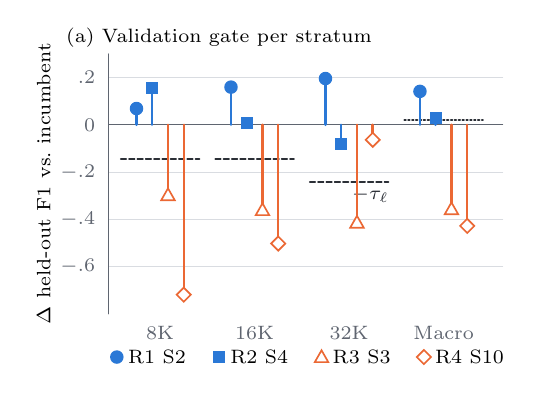
\begin{tikzpicture}[font=\scriptsize, line cap=round, baseline=0pt]
\draw[vizgrid, line width=0.3pt] (0,0.600) -- (5.000,0.600);
\node[anchor=east, text=vizink2] at (-0.05,0.600) {$-.6$};
\draw[vizgrid, line width=0.3pt] (0,1.200) -- (5.000,1.200);
\node[anchor=east, text=vizink2] at (-0.05,1.200) {$-.4$};
\draw[vizgrid, line width=0.3pt] (0,1.800) -- (5.000,1.800);
\node[anchor=east, text=vizink2] at (-0.05,1.800) {$-.2$};
\draw[vizgrid, line width=0.3pt] (0,2.400) -- (5.000,2.400);
\node[anchor=east, text=vizink2] at (-0.05,2.400) {0};
\draw[vizgrid, line width=0.3pt] (0,3.000) -- (5.000,3.000);
\node[anchor=east, text=vizink2] at (-0.05,3.000) {.2};
\draw[vizink2, line width=0.4pt] (0,2.400) -- (5.000,2.400);
\draw[vizink2, line width=0.4pt] (0,0) -- (0,3.300);
\draw[vizink, line width=0.6pt, dash pattern=on 2pt off 1pt] (0.150,1.969) -- (1.150,1.969);
\draw[vizink, line width=0.6pt, dash pattern=on 2pt off 1pt] (1.350,1.969) -- (2.350,1.969);
\draw[vizink, line width=0.6pt, dash pattern=on 2pt off 1pt] (2.550,1.669) -- (3.550,1.669);
\node[anchor=north east, text=vizink, inner sep=1pt] at (3.600,1.649) {$-\tau_\ell$};
\draw[vizink, line width=0.6pt, dash pattern=on 0.6pt off 0.8pt] (3.750,2.460) -- (4.750,2.460);
\draw[vizblue, line width=0.9pt] (0.350,2.400) -- (0.350,2.606);
\path[draw=vizblue, fill=vizblue, line width=0.6pt] (0.350,2.606) circle (0.075);
\draw[vizblue, line width=0.9pt] (1.550,2.400) -- (1.550,2.878);
\path[draw=vizblue, fill=vizblue, line width=0.6pt] (1.550,2.878) circle (0.075);
\draw[vizblue, line width=0.9pt] (2.750,2.400) -- (2.750,2.987);
\path[draw=vizblue, fill=vizblue, line width=0.6pt] (2.750,2.987) circle (0.075);
\draw[vizblue, line width=0.9pt] (3.950,2.400) -- (3.950,2.824);
\path[draw=vizblue, fill=vizblue, line width=0.6pt] (3.950,2.824) circle (0.075);
\draw[vizblue, line width=0.9pt] (0.550,2.400) -- (0.550,2.871);
\path[draw=vizblue, fill=vizblue, line width=0.6pt] (0.483,2.804) rectangle (0.618,2.938);
\draw[vizblue, line width=0.9pt] (1.750,2.400) -- (1.750,2.425);
\path[draw=vizblue, fill=vizblue, line width=0.6pt] (1.683,2.357) rectangle (1.817,2.492);
\draw[vizblue, line width=0.9pt] (2.950,2.400) -- (2.950,2.158);
\path[draw=vizblue, fill=vizblue, line width=0.6pt] (2.882,2.090) rectangle (3.017,2.225);
\draw[vizblue, line width=0.9pt] (4.150,2.400) -- (4.150,2.484);
\path[draw=vizblue, fill=vizblue, line width=0.6pt] (4.083,2.417) rectangle (4.218,2.552);
\draw[vizorange, line width=0.9pt] (0.750,2.400) -- (0.750,1.507);
\path[draw=vizorange, fill=white, line width=0.6pt] (0.750,1.593) -- (0.664,1.442) -- (0.836,1.442) -- cycle;
\draw[vizorange, line width=0.9pt] (1.950,2.400) -- (1.950,1.317);
\path[draw=vizorange, fill=white, line width=0.6pt] (1.950,1.403) -- (1.864,1.252) -- (2.036,1.252) -- cycle;
\draw[vizorange, line width=0.9pt] (3.150,2.400) -- (3.150,1.158);
\path[draw=vizorange, fill=white, line width=0.6pt] (3.150,1.244) -- (3.064,1.093) -- (3.236,1.093) -- cycle;
\draw[vizorange, line width=0.9pt] (4.350,2.400) -- (4.350,1.327);
\path[draw=vizorange, fill=white, line width=0.6pt] (4.350,1.414) -- (4.264,1.263) -- (4.436,1.263) -- cycle;
\draw[vizorange, line width=0.9pt] (0.950,2.400) -- (0.950,0.242);
\path[draw=vizorange, fill=white, line width=0.6pt] (0.950,0.332) -- (1.040,0.242) -- (0.950,0.152) -- (0.860,0.242) -- cycle;
\draw[vizorange, line width=0.9pt] (2.150,2.400) -- (2.150,0.892);
\path[draw=vizorange, fill=white, line width=0.6pt] (2.150,0.982) -- (2.240,0.892) -- (2.150,0.802) -- (2.060,0.892) -- cycle;
\draw[vizorange, line width=0.9pt] (3.350,2.400) -- (3.350,2.209);
\path[draw=vizorange, fill=white, line width=0.6pt] (3.350,2.299) -- (3.440,2.209) -- (3.350,2.119) -- (3.260,2.209) -- cycle;
\draw[vizorange, line width=0.9pt] (4.550,2.400) -- (4.550,1.115);
\path[draw=vizorange, fill=white, line width=0.6pt] (4.550,1.205) -- (4.640,1.115) -- (4.550,1.025) -- (4.460,1.115) -- cycle;
\node[anchor=north, text=vizink2] at (0.650,-0.03) {8K};
\node[anchor=north, text=vizink2] at (1.850,-0.03) {16K};
\node[anchor=north, text=vizink2] at (3.050,-0.03) {32K};
\node[anchor=north, text=vizink2] at (4.250,-0.03) {Macro};
\node[rotate=90, anchor=south] at (-0.62,1.650) {$\Delta$ held-out F1 vs.\ incumbent};
\node[anchor=south west, inner sep=0pt] at (-0.55,3.380) {(a) Validation gate per stratum};
\path[draw=vizblue, fill=vizblue, line width=0.6pt] (0.100,-0.550) circle (0.075);
\node[anchor=west, inner sep=1pt] at (0.200,-0.550) {R1 S2};
\path[draw=vizblue, fill=vizblue, line width=0.6pt] (1.333,-0.618) rectangle (1.468,-0.483);
\node[anchor=west, inner sep=1pt] at (1.500,-0.550) {R2 S4};
\path[draw=vizorange, fill=white, line width=0.6pt] (2.700,-0.464) -- (2.614,-0.615) -- (2.786,-0.615) -- cycle;
\node[anchor=west, inner sep=1pt] at (2.800,-0.550) {R3 S3};
\path[draw=vizorange, fill=white, line width=0.6pt] (4.000,-0.460) -- (4.090,-0.550) -- (4.000,-0.640) -- (3.910,-0.550) -- cycle;
\node[anchor=west, inner sep=1pt] at (4.100,-0.550) {R4 S10};
\end{tikzpicture}
\hfill
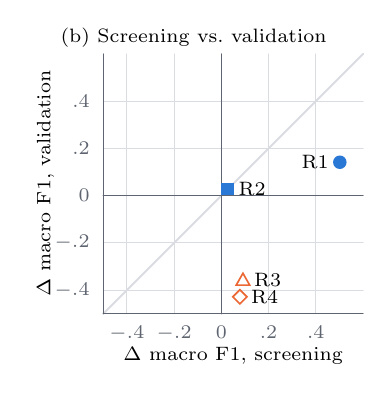
\begin{tikzpicture}[font=\scriptsize, line cap=round, baseline=0pt]
\draw[vizgrid, line width=0.3pt] (0,0.300) -- (3.300,0.300);
\draw[vizgrid, line width=0.3pt] (0.300,0) -- (0.300,3.300);
\node[anchor=east, text=vizink2] at (-0.05,0.300) {$-.4$};
\node[anchor=north, text=vizink2] at (0.300,-0.03) {$-.4$};
\draw[vizgrid, line width=0.3pt] (0,0.900) -- (3.300,0.900);
\draw[vizgrid, line width=0.3pt] (0.900,0) -- (0.900,3.300);
\node[anchor=east, text=vizink2] at (-0.05,0.900) {$-.2$};
\node[anchor=north, text=vizink2] at (0.900,-0.03) {$-.2$};
\draw[vizgrid, line width=0.3pt] (0,1.500) -- (3.300,1.500);
\draw[vizgrid, line width=0.3pt] (1.500,0) -- (1.500,3.300);
\node[anchor=east, text=vizink2] at (-0.05,1.500) {0};
\node[anchor=north, text=vizink2] at (1.500,-0.03) {0};
\draw[vizgrid, line width=0.3pt] (0,2.100) -- (3.300,2.100);
\draw[vizgrid, line width=0.3pt] (2.100,0) -- (2.100,3.300);
\node[anchor=east, text=vizink2] at (-0.05,2.100) {.2};
\node[anchor=north, text=vizink2] at (2.100,-0.03) {.2};
\draw[vizgrid, line width=0.3pt] (0,2.700) -- (3.300,2.700);
\draw[vizgrid, line width=0.3pt] (2.700,0) -- (2.700,3.300);
\node[anchor=east, text=vizink2] at (-0.05,2.700) {.4};
\node[anchor=north, text=vizink2] at (2.700,-0.03) {.4};
\draw[vizgrid, line width=0.7pt] (0,0) -- (3.300,3.300);
\draw[vizink2, line width=0.4pt] (0,1.500) -- (3.300,1.500);
\draw[vizink2, line width=0.4pt] (1.500,0) -- (1.500,3.300);
\draw[vizink2, line width=0.4pt] (0,0) -- (0,3.300) (0,0) -- (3.300,0);
\path[draw=vizblue, fill=vizblue, line width=0.6pt] (3.004,1.924) circle (0.075);
\node[anchor=east, inner sep=1pt] at (2.904,1.924) {R1};
\path[draw=vizblue, fill=vizblue, line width=0.6pt] (1.510,1.517) rectangle (1.645,1.652);
\node[anchor=west, inner sep=1pt] at (1.677,1.584) {R2};
\path[draw=vizorange, fill=white, line width=0.6pt] (1.774,0.514) -- (1.688,0.363) -- (1.860,0.363) -- cycle;
\node[anchor=west, inner sep=1pt] at (1.874,0.427) {R3};
\path[draw=vizorange, fill=white, line width=0.6pt] (1.735,0.305) -- (1.825,0.215) -- (1.735,0.125) -- (1.645,0.215) -- cycle;
\node[anchor=west, inner sep=1pt] at (1.835,0.215) {R4};
\node[rotate=90, anchor=south] at (-0.5,1.650) {$\Delta$ macro F1, validation};
\node[anchor=north] at (1.650,-0.3) {$\Delta$ macro F1, screening};
\node[anchor=south west, inner sep=0pt] at (-0.55,3.380) {(b) Screening vs.\ validation};
\end{tikzpicture}
\hfill
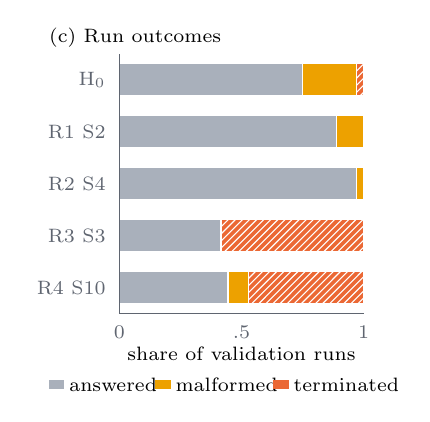
\begin{tikzpicture}[font=\scriptsize, baseline=0pt]
\path[fill=vizgrey, draw=white, line width=0.5pt] (0.000,2.765) rectangle (2.325,3.175);
\path[fill=vizyellow, draw=white, line width=0.5pt] (2.325,2.765) rectangle (3.014,3.175);
\path[fill=vizorange, draw=white, line width=0.5pt] (3.014,2.765) rectangle (3.100,3.175);
\begin{scope}\clip (3.014,2.765) rectangle (3.100,3.175);
\draw[white, line width=0.4pt] (2.605,2.765) -- (3.014,3.175);
\draw[white, line width=0.4pt] (2.695,2.765) -- (3.104,3.175);
\draw[white, line width=0.4pt] (2.785,2.765) -- (3.194,3.175);
\draw[white, line width=0.4pt] (2.875,2.765) -- (3.284,3.175);
\draw[white, line width=0.4pt] (2.965,2.765) -- (3.374,3.175);
\draw[white, line width=0.4pt] (3.055,2.765) -- (3.464,3.175);
\end{scope}
\node[anchor=east, text=vizink2] at (-0.05,2.970) {$\mathrm{H}_0$};
\path[fill=vizgrey, draw=white, line width=0.5pt] (0.000,2.105) rectangle (2.756,2.515);
\path[fill=vizyellow, draw=white, line width=0.5pt] (2.756,2.105) rectangle (3.100,2.515);
\node[anchor=east, text=vizink2] at (-0.05,2.310) {R1 S2};
\path[fill=vizgrey, draw=white, line width=0.5pt] (0.000,1.445) rectangle (3.014,1.855);
\path[fill=vizyellow, draw=white, line width=0.5pt] (3.014,1.445) rectangle (3.100,1.855);
\node[anchor=east, text=vizink2] at (-0.05,1.650) {R2 S4};
\path[fill=vizgrey, draw=white, line width=0.5pt] (0.000,0.785) rectangle (1.292,1.195);
\path[fill=vizorange, draw=white, line width=0.5pt] (1.292,0.785) rectangle (3.100,1.195);
\begin{scope}\clip (1.292,0.785) rectangle (3.100,1.195);
\draw[white, line width=0.4pt] (0.882,0.785) -- (1.292,1.195);
\draw[white, line width=0.4pt] (0.972,0.785) -- (1.382,1.195);
\draw[white, line width=0.4pt] (1.062,0.785) -- (1.472,1.195);
\draw[white, line width=0.4pt] (1.152,0.785) -- (1.562,1.195);
\draw[white, line width=0.4pt] (1.242,0.785) -- (1.652,1.195);
\draw[white, line width=0.4pt] (1.332,0.785) -- (1.742,1.195);
\draw[white, line width=0.4pt] (1.422,0.785) -- (1.832,1.195);
\draw[white, line width=0.4pt] (1.512,0.785) -- (1.922,1.195);
\draw[white, line width=0.4pt] (1.602,0.785) -- (2.012,1.195);
\draw[white, line width=0.4pt] (1.692,0.785) -- (2.102,1.195);
\draw[white, line width=0.4pt] (1.782,0.785) -- (2.192,1.195);
\draw[white, line width=0.4pt] (1.872,0.785) -- (2.282,1.195);
\draw[white, line width=0.4pt] (1.962,0.785) -- (2.372,1.195);
\draw[white, line width=0.4pt] (2.052,0.785) -- (2.462,1.195);
\draw[white, line width=0.4pt] (2.142,0.785) -- (2.552,1.195);
\draw[white, line width=0.4pt] (2.232,0.785) -- (2.642,1.195);
\draw[white, line width=0.4pt] (2.322,0.785) -- (2.732,1.195);
\draw[white, line width=0.4pt] (2.412,0.785) -- (2.822,1.195);
\draw[white, line width=0.4pt] (2.502,0.785) -- (2.912,1.195);
\draw[white, line width=0.4pt] (2.592,0.785) -- (3.002,1.195);
\draw[white, line width=0.4pt] (2.682,0.785) -- (3.092,1.195);
\draw[white, line width=0.4pt] (2.772,0.785) -- (3.182,1.195);
\draw[white, line width=0.4pt] (2.862,0.785) -- (3.272,1.195);
\draw[white, line width=0.4pt] (2.952,0.785) -- (3.362,1.195);
\draw[white, line width=0.4pt] (3.042,0.785) -- (3.452,1.195);
\end{scope}
\node[anchor=east, text=vizink2] at (-0.05,0.990) {R3 S3};
\path[fill=vizgrey, draw=white, line width=0.5pt] (0.000,0.125) rectangle (1.378,0.535);
\path[fill=vizyellow, draw=white, line width=0.5pt] (1.378,0.125) rectangle (1.636,0.535);
\path[fill=vizorange, draw=white, line width=0.5pt] (1.636,0.125) rectangle (3.100,0.535);
\begin{scope}\clip (1.636,0.125) rectangle (3.100,0.535);
\draw[white, line width=0.4pt] (1.227,0.125) -- (1.636,0.535);
\draw[white, line width=0.4pt] (1.317,0.125) -- (1.726,0.535);
\draw[white, line width=0.4pt] (1.407,0.125) -- (1.816,0.535);
\draw[white, line width=0.4pt] (1.497,0.125) -- (1.906,0.535);
\draw[white, line width=0.4pt] (1.587,0.125) -- (1.996,0.535);
\draw[white, line width=0.4pt] (1.677,0.125) -- (2.086,0.535);
\draw[white, line width=0.4pt] (1.767,0.125) -- (2.176,0.535);
\draw[white, line width=0.4pt] (1.857,0.125) -- (2.266,0.535);
\draw[white, line width=0.4pt] (1.947,0.125) -- (2.356,0.535);
\draw[white, line width=0.4pt] (2.037,0.125) -- (2.446,0.535);
\draw[white, line width=0.4pt] (2.127,0.125) -- (2.536,0.535);
\draw[white, line width=0.4pt] (2.217,0.125) -- (2.626,0.535);
\draw[white, line width=0.4pt] (2.307,0.125) -- (2.716,0.535);
\draw[white, line width=0.4pt] (2.397,0.125) -- (2.806,0.535);
\draw[white, line width=0.4pt] (2.487,0.125) -- (2.896,0.535);
\draw[white, line width=0.4pt] (2.577,0.125) -- (2.986,0.535);
\draw[white, line width=0.4pt] (2.667,0.125) -- (3.076,0.535);
\draw[white, line width=0.4pt] (2.757,0.125) -- (3.166,0.535);
\draw[white, line width=0.4pt] (2.847,0.125) -- (3.256,0.535);
\draw[white, line width=0.4pt] (2.937,0.125) -- (3.346,0.535);
\draw[white, line width=0.4pt] (3.027,0.125) -- (3.436,0.535);
\end{scope}
\node[anchor=east, text=vizink2] at (-0.05,0.330) {R4 S10};
\draw[vizink2, line width=0.4pt] (0,0) -- (3.100,0) (0,0) -- (0,3.300);
\node[anchor=north, text=vizink2] at (0.000,-0.03) {0};
\node[anchor=north, text=vizink2] at (1.550,-0.03) {.5};
\node[anchor=north, text=vizink2] at (3.100,-0.03) {1};
\node[anchor=north] at (1.550,-0.3) {share of validation runs};
\node[anchor=south west, inner sep=0pt] at (-0.9,3.380) {(c) Run outcomes};
\path[fill=vizgrey] (-0.900,-0.960) rectangle (-0.700,-0.840);
\node[anchor=west, inner sep=1pt] at (-0.680,-0.900) {answered};
\path[fill=vizyellow] (0.450,-0.960) rectangle (0.650,-0.840);
\node[anchor=west, inner sep=1pt] at (0.670,-0.900) {malformed};
\path[fill=vizorange] (1.950,-0.960) rectangle (2.150,-0.840);
\node[anchor=west, inner sep=1pt] at (2.170,-0.900) {terminated};
\end{tikzpicture}
\caption{Pilot run (DeepSeek-V4-Flash, OOLONG-Pairs, 12 validation tasks
$\times$ 3 attempts per subject). Filled blue markers are promoted
candidates and hollow orange markers are rejected ones; R$t$~S$j$ is the round
and edited surface. (a)~Held-out F1 change against the round's incumbent per
stratum and macro-averaged. Dashed lines are the veto margins $-\tau_\ell$; the
dotted line is $\tau_{\mathrm{imp}}$. (b)~Macro-F1 change in screening (3 tasks
$\times$ 1 attempt) against full validation; the grey line is $y{=}x$.
(c)~Outcome of the 36 validation runs: a scored answer, a malformed answer
(\texttt{wrong\_format}, F1 $=0$), or termination by the 3,600\,s cap (F1
$=0$). Incumbent rows after round 1 reuse the previous candidate's runs and
are omitted.}
\label{fig:pilot}
\end{figure*}
